\documentclass[../report.tex]{subfiles}
\begin{document}
\subsection{Sơ đồ khối và tín hiệu}
\begin{figure}[H]
    \centering
    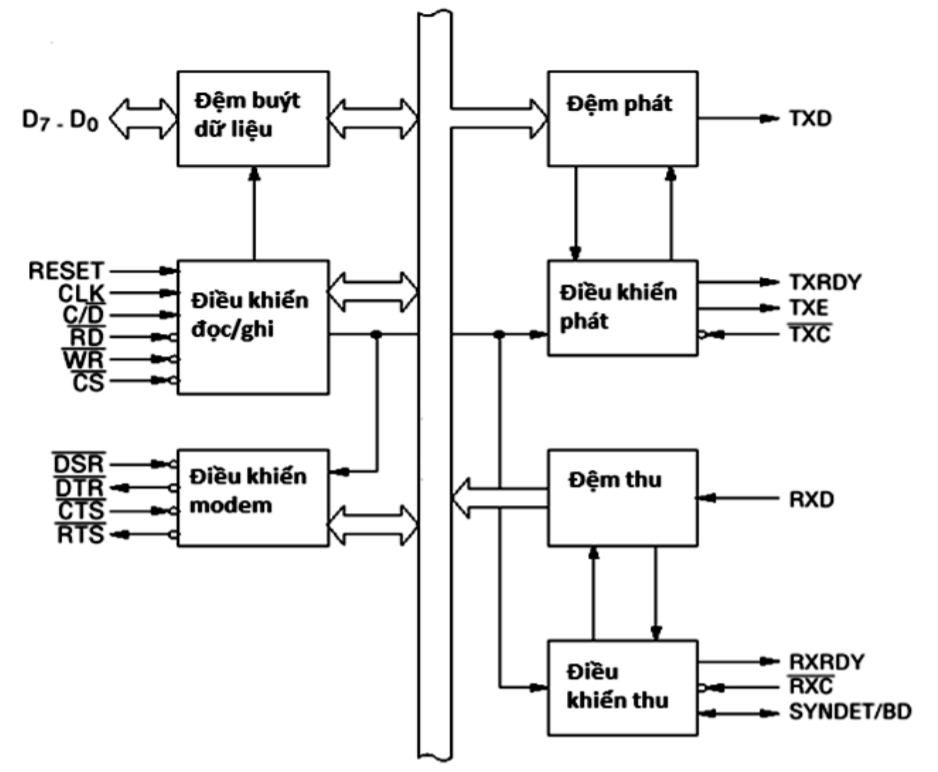
\includegraphics[width=\textwidth]{figures/8251.png}
    \caption{Sơ đồ khối 8251A}
\end{figure}
Các tín hiệu của mạch 8251A hầu hết là giống tín hiệu của 8086. Chân chọn vỏ của
8251A phải được nối với đầu ra của một mạch giải mã địa chỉ để đặt mạch 8251A vào một
địa chỉ cơ bản nào đó.
\begin{itemize}
    \item  CLK [I]: Chân nối đến xung đồng hồ của hệ thống.
    \item  TxRDY [0]: Tín hiệu báo đệm giữ rỗng (sẵn sàng nhận ký tự mới từ CPU).
    \item  RxRDY [0]: Tín hiệu báo đệm thu đầy (có ký hiệu nằm chờ CPU đọc vào).
    \item TxEMPTY [0]: Tín hiệu báo cả đệm thu và đệm phát đều rỗng. 
    \item C/D [I]: CPU thao tác với thanh ghi lệnh/thanh ghi dữ liệu của 8251A, khi C/D=1 thì
thanh ghi lệnh được chọn làm việc. Chân này thường được nối với A0 của bus địa chỉ để cùng
với các tín hiệu WR và RD chọn ra 4 thanh ghi bên trong 8251A. 
    \item  RxC [I] và TxC [I]: Xung đồng hồ cung cấp cho các thanh ghi dịch của phần thu và
phần phát. Thường 2 thanh này nối chung để phần thu và phần phát làm việc với cùng tầng số
nhịp. Tần số của các khung đồng hồ đưa đến chân RxC và TxC được chọn sao cho là bội số
(cụ thể là gấp 1, 16 hoặc 64) của tốc độ thu hay tốc độ phát theo yêu cầu. 
    \item DSR, DTR: là cặp tín hiệu yêu cầu thiết bị modem sẵn sàng và trả lời của modem với tín hiệu yêu cầu. 
    \item RTS, CTS:  là cặp tín hiệu yêu cầu modem sẵn sàng phát và đáp ứng của modem với tín hiệu yêu cầu. 
    \item SYNDET/BRKDET [O]: khi 8251A làm việc ở chế độ không đồng bộ, nếu RxD = 0
kéo dài hơn thời gian của 2 ký tự thì chân này có mức cao để báo là việc truyền hoặc đường
truyền bị gián đoạn. Khi 8251A làm việc ở chế độ đồng bộ, nếu phần thu tìm thấy ký tự đồng
bộ rong bản tin thu được thì chân này có mức cao.
\end{itemize}

\subsection{Các thanh ghi bên trong}
\subsubsection{Thanh ghi lệnh}
Cấu trúc thanh ghi lệnh như sau:
\begin{figure}[H]
    \centering
    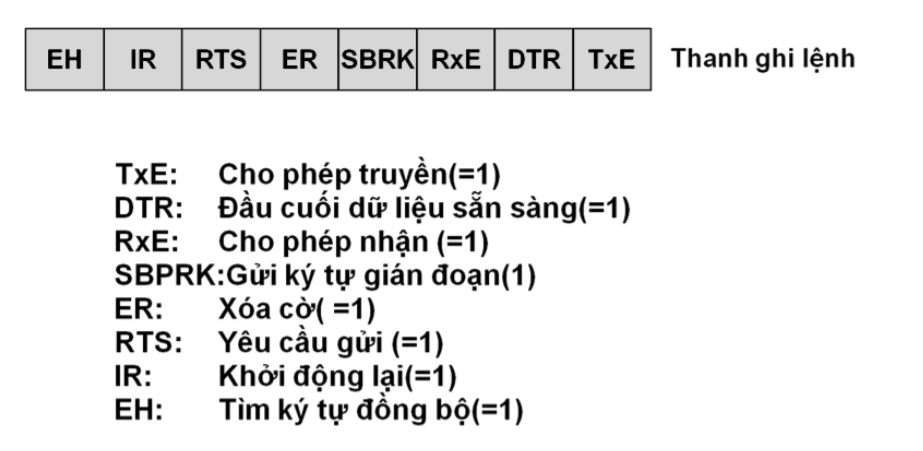
\includegraphics[width=\textwidth]{figures/lenh.png}
    \caption{Cấu trúc thanh ghi lệnh}
\end{figure}


\subsubsection{Thanh ghi trạng thái}
Giá trị trên các bít thanh ghi này cho ta biết tình trạng hoạt động của 8251A.
\begin{figure}[H]
    \centering
    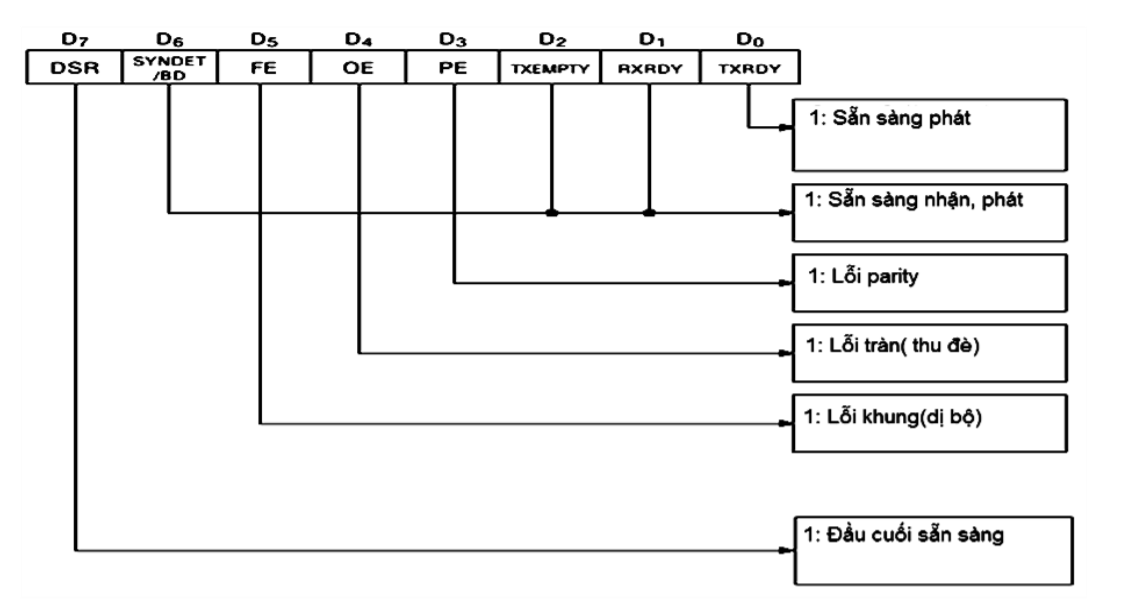
\includegraphics[width=\textwidth]{figures/trangthai.png}
    \caption{Cấu trúc thanh ghi trạng thái}
\end{figure}

\newpage
\subsection{Lập trình 8251A}
Để lập trình cho 8251A trước tiên ta cần xác lập chế độ hoạt động bằng cách tính giá trị
của thanh ghi chế độ và gửi ra cổng điều khiển. Để gửi hoặc nhận dữ liệu ta cần liên tục kiểm
tra trạng thái của 8251A theo lưu đồ đọc/ghi đơn giản sau:
\begin{figure}[H]
    \centering
    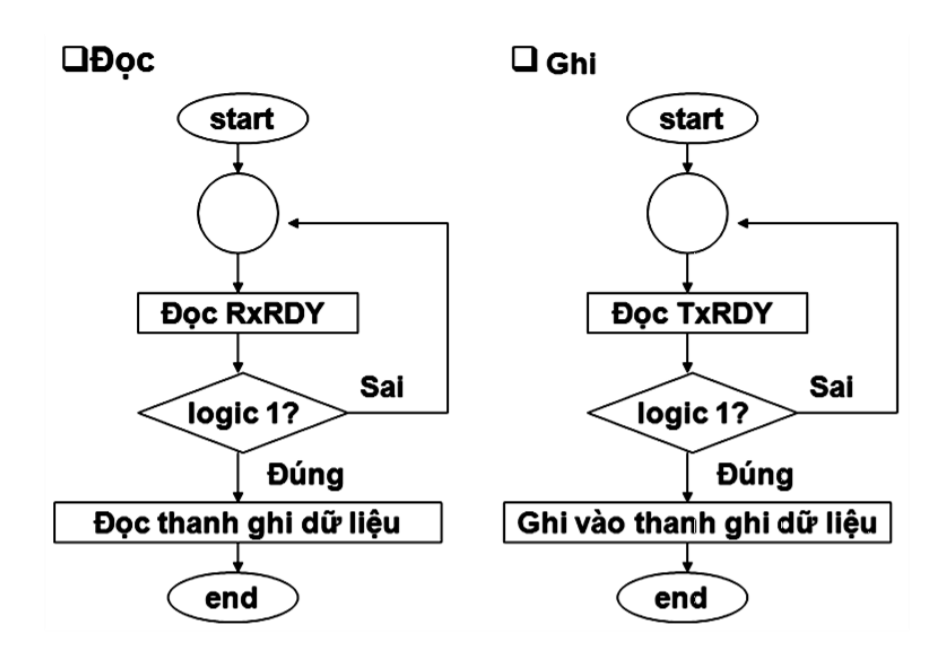
\includegraphics[width=\textwidth]{figures/io.png}
    \caption{Lưu đồ đọc ghi đơn giản}
\end{figure}
\end{document}
